\documentclass[../../main.tex]{subfiles}

\begin{document}

\subsubsection*{Auswertung Kenntnisse zu Sicherheitsthemen}
\addcontentsline{toc}{subsubsection}{Auswertung Kenntnisse zu Sicherheitsthemen}

\subparagraph*{Frage: Kann gesicherte Verbindung im Browser erkennen}\mbox{}
\begin{figure}[H]
\centering
\framebox[\textwidth]{\scriptsize $n: 253$}
\framebox[\textwidth]{\scalebox{0.9}{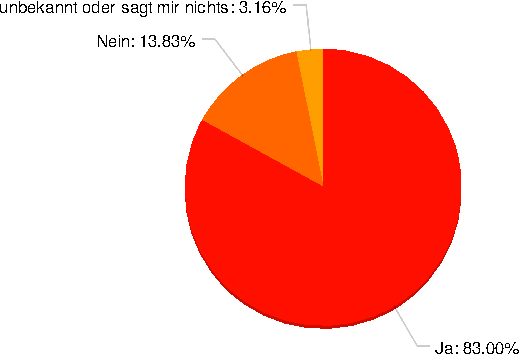
\includegraphics{figures/esurvey/c_ver_v28_secure_webaccess}}}
\caption{Auswertung Frage V28}
\label{V28}
\end{figure}

\subparagraph*{Frage: Email ist ein sicherer Datenübertragungsweg}\mbox{}
\begin{figure}[H]
\centering
\framebox[\textwidth]{\scriptsize 0 = Trifft überhaupt nicht zu $\vert$ 100 = Trifft voll zu ($n: 253$, $\bar{x}: 20.60$, $\sigma: 25.52$)}
\framebox[\textwidth]{\scalebox{0.9}{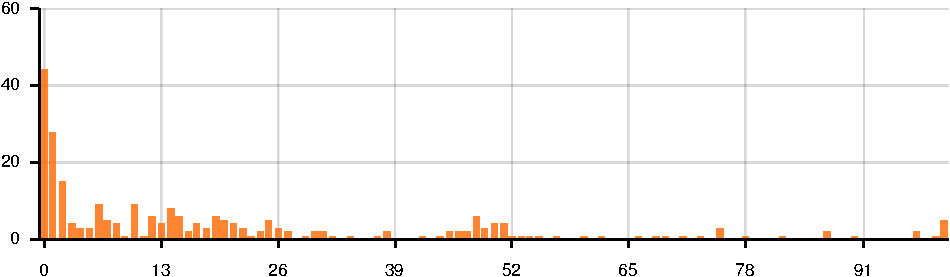
\includegraphics{figures/esurvey/c_ver_v29_email_security}}}
\caption{Auswertung Frage V29}
\label{V29}
\end{figure}

\subparagraph*{Frage: Gelöschte Daten können wiederhergestellt werden}\mbox{}
\begin{figure}[H]
\centering
\framebox[\textwidth]{\scriptsize $n: 253$}
\framebox[\textwidth]{\scalebox{0.9}{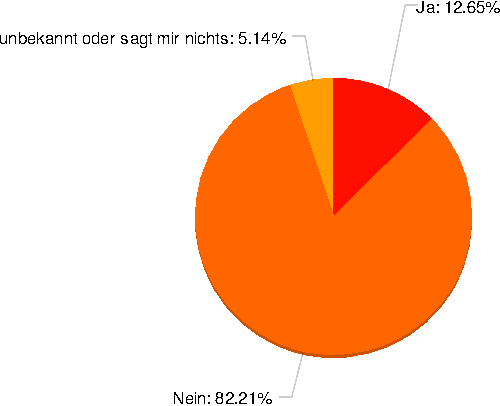
\includegraphics{figures/esurvey/c_ver_v30_delete_data}}}
\caption{Auswertung Frage V30}
\label{V30}
\end{figure}

\subparagraph*{Frage: Kann Zwei-Faktor Authentisierung erklären}\mbox{}
\begin{figure}[H]
\centering
\framebox[\textwidth]{\scriptsize 0 = Trifft überhaupt nicht zu $\vert$ 100 = Trifft voll zu ($n: 253$, $\bar{x}: 70.47$, $\sigma: 35.09$)}
\framebox[\textwidth]{\scalebox{0.9}{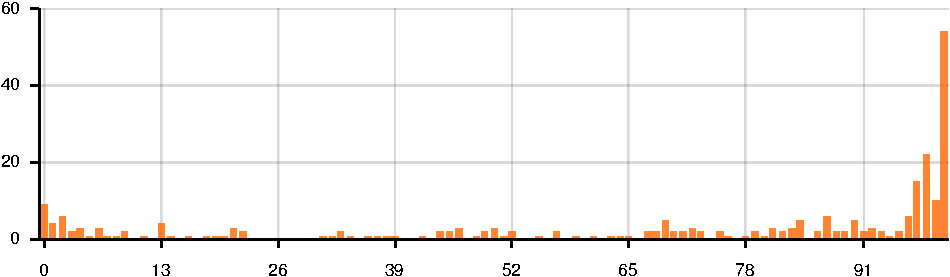
\includegraphics{figures/esurvey/c_ver_v31_two_factor}}}
\caption{Auswertung Frage V31}
\label{V31}
\end{figure}

\subparagraph*{Frage: Kann Phishing E-Mails erkennen}\mbox{}
\begin{figure}[H]
\centering
\framebox[\textwidth]{\scriptsize 0 = Trifft überhaupt nicht zu $\vert$ 100 = Trifft voll zu ($n: 253$, $\bar{x}: 74.60$, $\sigma: 24.65$)}
\framebox[\textwidth]{\scalebox{0.9}{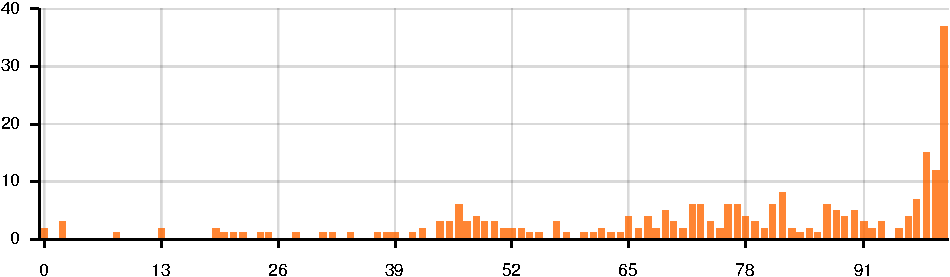
\includegraphics{figures/esurvey/c_ver_v32_phishing}}}
\caption{Auswertung Frage V32}
\label{V32}
\end{figure}

\subparagraph*{Frage: Kann Begriff "Ransomware" erklären}\mbox{}
\begin{figure}[H]
\centering
\framebox[\textwidth]{\scriptsize 0 = Trifft überhaupt nicht zu $\vert$ 100 = Trifft voll zu ($n: 253$, $\bar{x}: 56.87$, $\sigma: 41.30$)}
\framebox[\textwidth]{\scalebox{0.9}{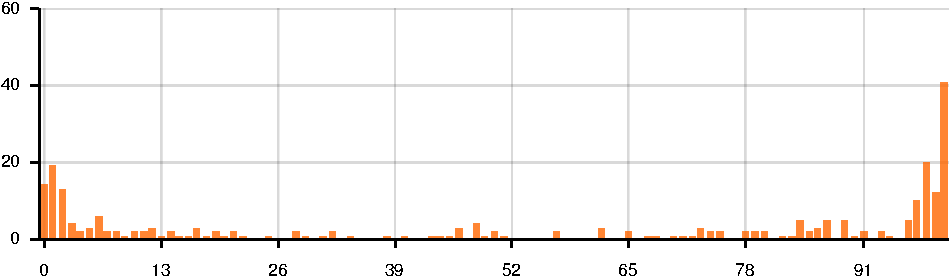
\includegraphics{figures/esurvey/c_ver_v33_ransomware}}}
\caption{Auswertung Frage V33}
\label{V33}
\end{figure}

\subparagraph*{Frage: Kann Begriff "Social Engineering" erklären}\mbox{}
\begin{figure}[H]
\centering
\framebox[\textwidth]{\scriptsize 0 = Trifft überhaupt nicht zu $\vert$ 100 = Trifft voll zu ($n: 253$, $\bar{x}: 66.28$, $\sigma: 35.56$)}
\framebox[\textwidth]{\scalebox{0.9}{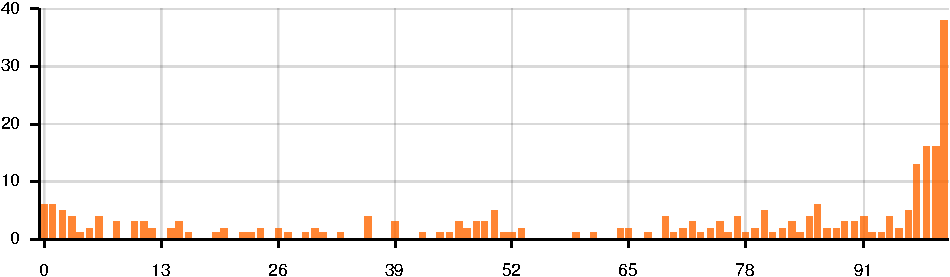
\includegraphics{figures/esurvey/c_ver_v34_social_engineering}}}
\caption{Auswertung Frage V34}
\label{V34}
\end{figure}


\end{document}
